\documentclass[tikz]{standalone}
\usepackage{tikz}
\usetikzlibrary{shapes, arrows.meta, positioning, backgrounds, fit, calc}

\begin{document}
    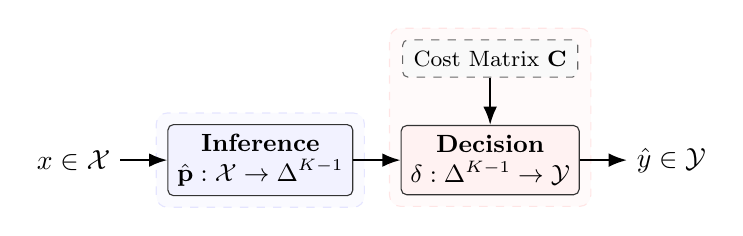
\begin{tikzpicture}[
        node distance=0.6cm,
        auto,
        block/.style={
            rectangle, 
            draw=black!80, 
            fill=blue!5, 
            align=center, 
            rounded corners=2pt, 
            minimum height=2.5em,
            minimum width=2.2cm,
            font=\small\bfseries
        },
        decision/.style={
            rectangle, 
            draw=black!80, 
            fill=red!5, 
            align=center, 
            rounded corners=2pt, 
            minimum height=2.5em,
            minimum width=2.2cm,
            font=\small\bfseries
        },
        param/.style={
            rectangle,
            draw=black!60,
            dashed,
            fill=gray!5,
            rounded corners=2pt,
            font=\footnotesize,
            inner sep=4pt
        },
        line/.style={
            draw, 
            -Latex, 
            thick
        }
    ]

        % --- Nodes ---
        
        \node (input) {$x \in \mathcal{X}$};

        \node [block, right=of input] (model) {\textbf{Inference} \\ $\hat{\mathbf{p}}: \mathcal{X} \to \Delta^{K-1}$};
        
        \node [decision, right=of model] (delta) {\textbf{Decision} \\ $\delta: \Delta^{K-1} \to \mathcal{Y}$};
        
        \node [right=of delta] (output) {$\hat{y} \in \mathcal{Y}$};
        
        \node [param, above=0.6cm of delta] (cost) {Cost Matrix $\mathbf{C}$};

        % --- Background Groups ---
        \begin{scope}[on background layer]
            \node [fit=(model), fill=blue!2, draw=blue!10, dashed, rounded corners, inner sep=4pt] {};
            \node [fit=(delta) (cost), fill=red!2, draw=red!10, dashed, rounded corners, inner sep=4pt] {};
        \end{scope}

        % --- Edges ---
        \path [line] (input) -- (model);
        \path [line] (model) -- (delta);
        \path [line] (delta) -- (output);
        \path [line] (cost) -- (delta);

    \end{tikzpicture}
\end{document}